% continue here, noisy graphs ready to run

\section{Evaluation}  \label{sec:evaluation}

\subsection{Qualitative Comparison} \label{sec:qual_comp}
The control law presented was tested in simulation in Python. The state space is the Cartesian coordinates $xy$ in 2D and $xyz$ in 3D. In practice, the damping matrix $\matd D(\vecs\xi)$ and the control command $\vecs {\tau_c}$ are recomputed at each time step.\\

Let us compare traditional passive interaction control and the presented method (Fig.~\ref{fig_diff_obs_pass}). On the setup, the same disturbance is applied to both systems simultaneously. One can already see the robot equipped with traditional passive control (left) penetrates the obstacle, while ours (right) successfully damps the disturbance.

% \begin{figure}
% \centering
% \begin{subfigure}{0.8\columnwidth}
%   \centerline{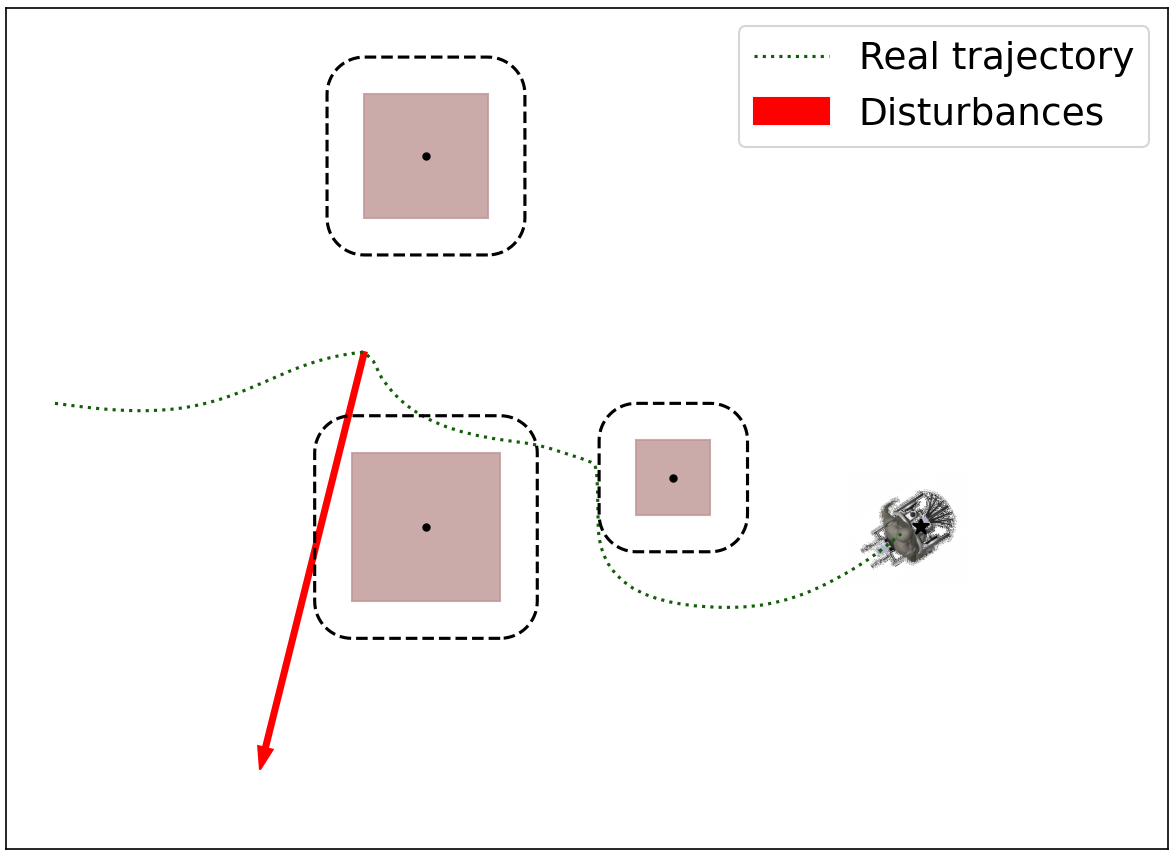
\includegraphics[width=\textwidth]{figures/run_without_pass.png}}
%   \caption{Traditional passive control}
% \end{subfigure}
% \begin{subfigure}{0.8\columnwidth}
%   \centerline{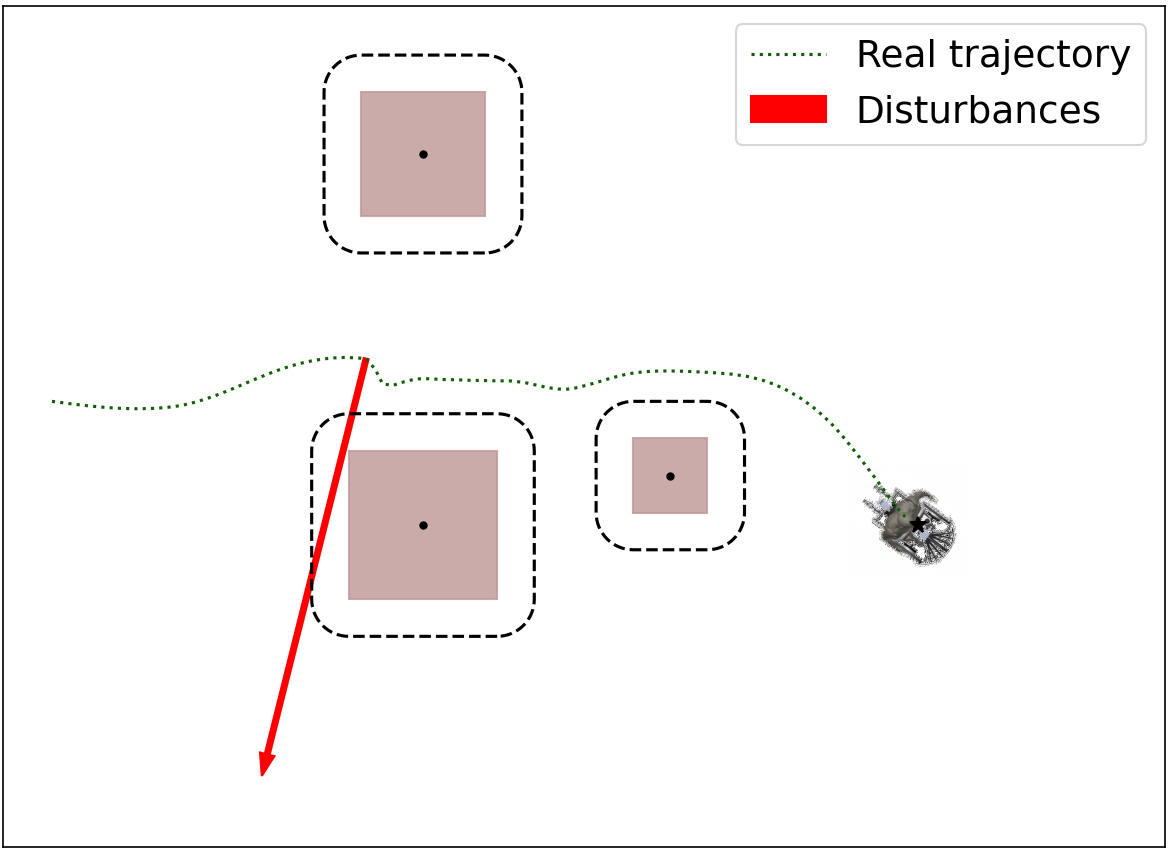
\includegraphics[width=\textwidth]{figures/run_with_pass.png}}
%   \caption{Obstacle aware passive control}
% \end{subfigure}
% \caption{Comparison of the two control methods}
% \label{fig:diff_obs_pass}
% \end{figure}

\begin{figure}
  \centering
  \centerline{\includesvg{}[width=0.95\columnwidth]{figures/multi_obstacle_with_damping.svg}}
  % \centerline{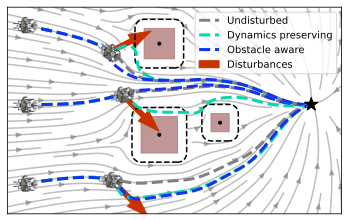
\includegraphics[width=0.5\textwidth]{figures/multi_obstacle_with_damping.svg}}
  \caption{The desired dynamics $\dot{\vecs \xi}$ in gray are as input for the force controller. 
  The mobile robot starting from the three positions, navigates safely to the attractor (black star) despite the disturbances (red arrows) when using the obstacle-aware controller.
  Conversely, the baseline (blue) leads to collision when the disturbance happens close to the robot.}
  \label{fig:obstacle_aware_damping_comparison}
\end{figure}

\subsection{Comparison to Reference Trajectory}
We will now look at the performance of our controller in different scenarios. Fig.~\ref{fig_run_with_obs} shows a simulation with 3 obstacles. The red arrows represent manually applied disturbances. The ideal trajectory is also displayed (perfect DS tracking, not subjected to real dynamics). Based on this simulation, we can observe the robots' behavior in different scenarios.

The first disturbance (A) pushed the robot in a direction perpendicular to the desired motion. Since we want compliance in this direction and the robot is far from any obstacle, it deviates greatly from its previous trajectory. It continues its path to the attractor on another DS line.

Another disturbance (B) pushed the robot toward the obstacle and was successfully damped, avoiding the collision.

A disturbance (C) pushed the robot away from an obstacle. The control algorithm is made such that when moving away from an obstacle, disturbances are not damped, and the robot shows compliant behavior. 

The last disturbance (D) was applied along the direction of motion. As the desired behavior is stiff in this direction, the robot almost kept the same speed and continued toward the attractor.

% \begin{figure}
% \centerline{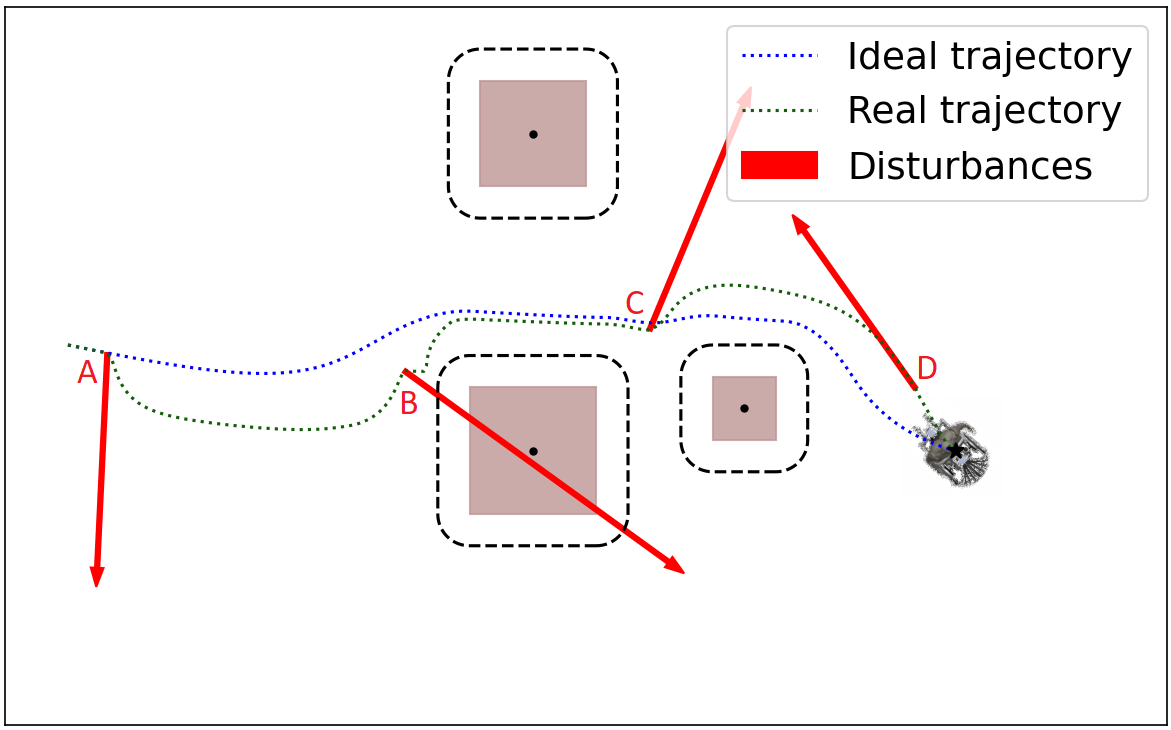
\includegraphics[width=0.5\textwidth]{figures/run_with_obs.png}}
% \caption{Simulation with a complex environment and disturbances applied to the robot}
% \label{fig_run_with_obs}
% \end{figure}

Furthermore, in Fig.~\ref{fig_run_damped_towards}, one can observe the feature described in Section~\ref{sec:damping_only_toward}, that only damps the disturbance towards the obstacle.
The first disturbance is highly damped, while the second is much less. This feature provides a natural behavior of moving away from obstacles, improving the margin of impenetrability. 

\subsection{Noise analysis}
Gaussian noise was added to the simulation to assert the control law's robustness. We added two types of noise, noise on the position measurements and noise on the velocity measurements. 

The experiment is done on a simple setup with one obstacle. The noise added has a mean of $0$, and the standard deviation is increasing linearly from $0.0$ to $0.7m$ for position and $0.0$ to $7.0 \frac{m}{s}$ for velocity measurements. For each noise level, the simulation was run 10 times. The output variable is the smallest distance of the agent from the obstacle during the simulation. This metric was chosen to observe how the noise could lead to a crash in the obstacle. 

For the noise acting on the position measurement, the controller presents good rejection for a small noise variance. As it increases, the robot's behavior quickly worsens (Fig.~\ref{fig_pos_noise}). The robot penetrates the obstacle for noises of standard deviation $ > 0.4 m$. An example of a run with $\sigma_{noise} = 0.7 m$ is shown in Fig.~\ref{fig_pos_noise_0_7}.

\begin{figure}
\centerline{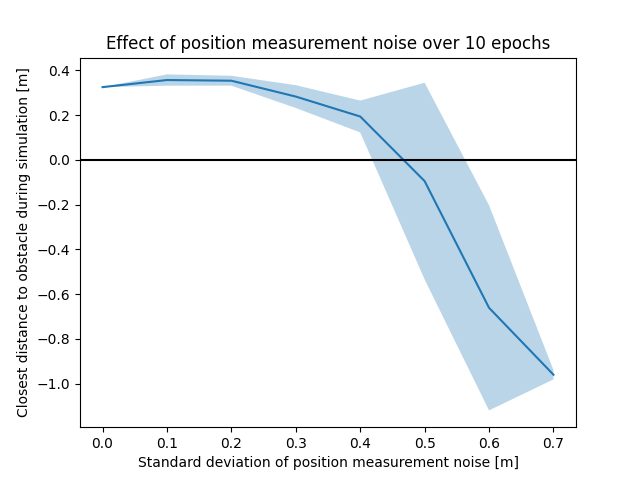
\includegraphics[width=0.5\textwidth]{figures/noise_pos_v2.png}}
\caption{Noise on the position measurements (shaded region are within one standard deviation from the mean)}
\label{fig_pos_noise}
\end{figure}

\begin{figure}
\centerline{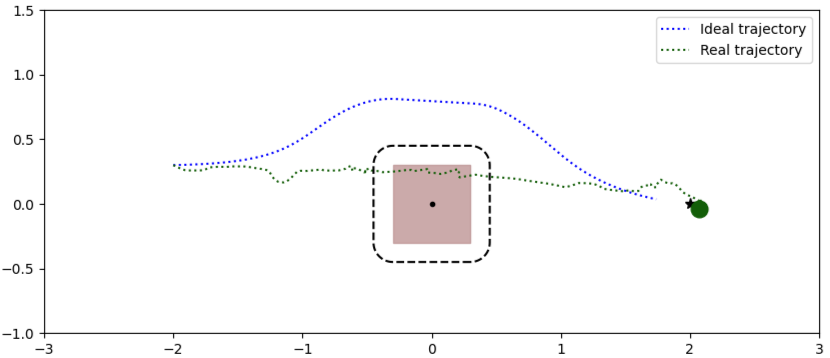
\includegraphics[width=0.5\textwidth]{figures/noise_effect_0_7.png}}
\caption{Noise on the position measurement with a standard deviation of 0.7 $m$ (with ideal trajectory displayed)}
\label{fig_pos_noise_0_7}
\end{figure}

The obstacle was never penetrated for the velocity measurement noise, asserting the robustness of the control for this type of noise (Fig.~\ref{fig_vel_noise}). Fig.~\ref{fig_2_vel_noise} provides an image of the simulation with big noise standard deviation ($4.0 \frac{m}{s}$). Thanks to the feature presented in Section~\ref{sec:damping_only_toward} (damping only toward the obstacle), the robot has even the tendency to drift away from the obstacle, increasing the safety margin.


\begin{figure}
    \centering
    \begin{subfigure}{\columnwidth}
      \centerline{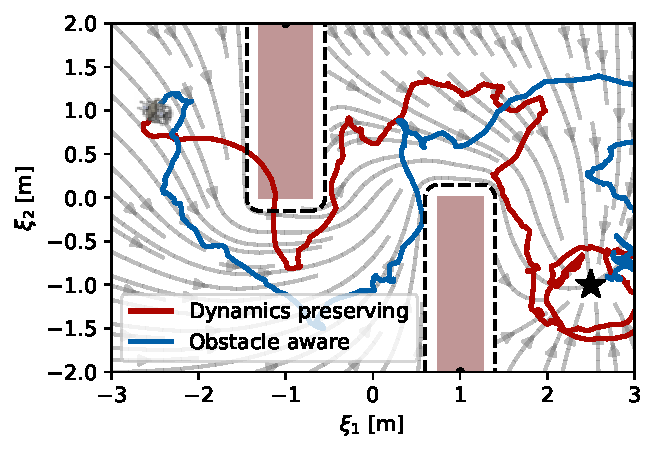
\includegraphics[width=\textwidth]{figures/trajectory_velocity_noise}}
      \caption{A single trajectory with a standard deviation of the noise level of 1.0 m/s.}
      \label{fig:trajectory_velocity_noise}
    \end{subfigure}
    \begin{subfigure}{\columnwidth}
    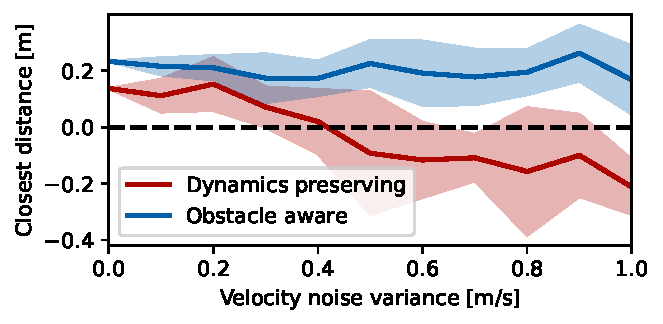
\includegraphics[width=\textwidth]{figures/comparison_velocity_noise}
      \caption{Closest distances concerning different noise levels over 10 epochs.}
      \label{fig:comparison_velocity_noise}
    \end{subfigure}
    \caption{}
\label{fig:velocity_noise}
\end{figure}


\begin{figure}
\centerline{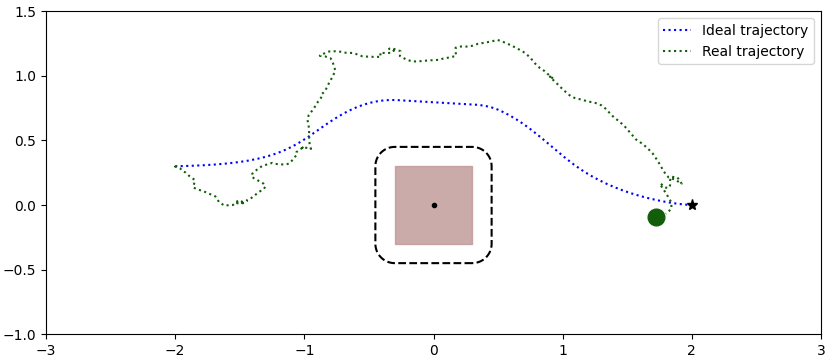
\includegraphics[width=\columnwidth]{figures/vel_noise_4.0.png}}
\caption{A simulation with noise on the velocity measurement with a standard deviation of $4.0 \frac{m}{s}$  (with ideal trajectory displayed)}
\label{fig_2_vel_noise}
\end{figure}


\subsection{Evaluation on Robot Arm}

\begin{figure}
    \centering
    \begin{subfigure}{\columnwidth}
      \centerline{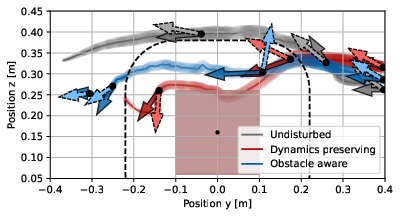
\includegraphics[width=\textwidth]{figures/robot_arm_trajectory_xyz}}
      \caption{Parallel to surface velocity}
      \label{fig:robot_arm_trajectory_xyz}
    \end{subfigure}
    \begin{subfigure}{\columnwidth}
    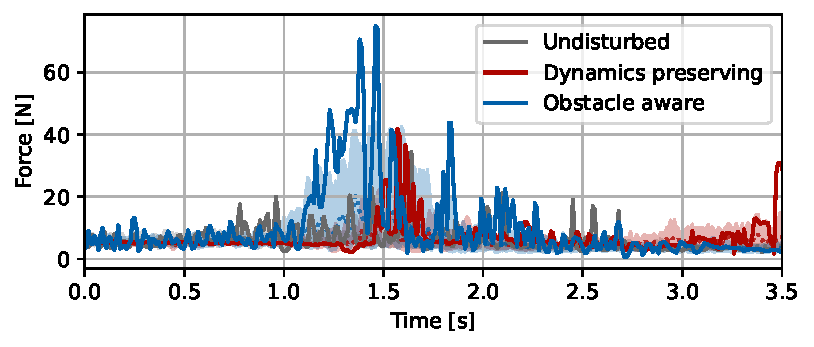
\includegraphics[width=\textwidth]{figures/trajectory_comparison_force_magnitude}
      \caption{Repulsive surface velocity}
      \label{fig:trajectory_comparison_force_magnitude}
    \end{subfigure}
    \begin{subfigure}{\columnwidth}
       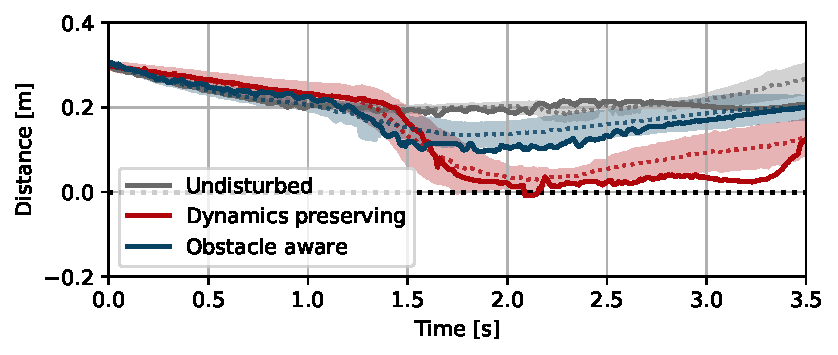
\includegraphics[width=\textwidth]{figures/robot_arm_trajectory_distance}
      \caption{Repulsive surface velocity}
      \label{fig:disturbance_with_repulsive_velocity}
    \end{subfigure}
    \caption{Comparison of the two control methods}
    \label{fig:evaluation_on_robot_arm}
\end{figure}

\section{Discussion}
Overall, the simulated robot shows pleasing results. It has good tracking performances, compliance in the direction perpendicular to the motion, and great damping of the disturbances towards obstacles.
Away from obstacles, the controller presented shows similar behavior as the one in \cite{kronander2015passive}. When approaching one obstacle, the control gets stiffer to avoid collisions without losing its tracking properties. This makes the proposed controller a suitable option to cumulate good tracking and safety regarding obstacle penetration.

\subsection{Applicability Approach}
Note, that the theoretical analysis from Theorem~\ref{theorem:passivity}, indicates passivity for any velocity-bounded, uniquely damped system. As a result, work such as the damping-based controller in  \cite{kronander2015passive} does not require an energy tank anymore.
Conversely, if the impedance controller has a proportional $\mathcal{K}$, the adaptive proportional term might induce instabilities even for stable desired dynamics as pointed out in \cite{ferraguti2013tank, kronander2016stability}.